\documentclass{beamer}

\setlength{\unitlength}{1cm} 
\usetheme{Madrid}

\usepackage[english]{babel}
\usepackage[utf8]{inputenc}

\usepackage{amsmath, amssymb, mathtools, bbm}
\usepackage{bm}

\usepackage{graphicx}
\usepackage{wrapfig}
\usepackage{tikz} 
\usepackage{relsize}
\usepackage{makecell}
\usepackage{booktabs}
\usepackage{subcaption}
\usepackage{float}
\usepackage{multirow} 

\usepackage[style=apa]{biblatex}
\usepackage{csquotes}

\bibliography{
    ../../../../Desktop/bibliographies/thesis,
    ../maths}


% Graphs
\usetikzlibrary{positioning, arrows.meta, calc, decorations.markings, math, matrix, fit, backgrounds}

\tikzset{fontscale/.style = {font=\relscale{#1}}}

\definecolor{prosumer}{cmyk}{0,0.816,0.408,0}

% Math commands
\newcommand{\E}{\mathbb{E}}
\newcommand{\R}{\mathbb{R}}
\newcommand{\B}{\mathbb{B}}

\newcommand{\matr}[1]{\bm{#1}}
\newcommand{\set}[1]{\left\{#1\right\}}

\newcommand{\Y}{\matr{Y}}
\newcommand{\I}{\matr{I}}
\newcommand{\G}{\matr{G}}
\newcommand{\T}{\matr{T}}

\title{How directed is a directed network?}
\author{Andrea Titton}
\title{Thesis defence}
\subtitle{Contagion of Electricity Prices \\ A Dynamic Game of Price Hikes Propagation}
\institute{Tinbergen Institute}
\date{04/12/2020}

\begin{document}

\frame{\titlepage}

\begin{frame}{Motivation}
    Green energy transition and advent of prosumers
    \vspace{2em}
    \begin{itemize}\setlength\itemsep{1.5em}
        \item \textbf{Electricity production} becomes prerogative of households
        \item \textbf{Local quasi-monopolies} energy providers (e.g. ERCOT case in Texas) and decentralized prosumers
        \item Weather shocks lead to \textbf{uncertainty} among risk averse consumers
    \end{itemize}
\end{frame}

\begin{frame}{Research question}

    Prosumers induce three sources of uncertainty: bounded rationality, risk aversion, and renewable energy volatility

    \begin{itemize} \setlength{\itemsep}{1em}
        \item \textit{What are the consequences for stability and prices in the wholesale cross-border daily electricity market?}
        \item \textit{Is the current strategy of further integration (EU and USA) the best one?}
        \item \textit{Can the system be stable without ``traditional'' producers?}
    \end{itemize}

\end{frame}

\begin{frame}{Lack of price convergence}
    \begin{figure}
        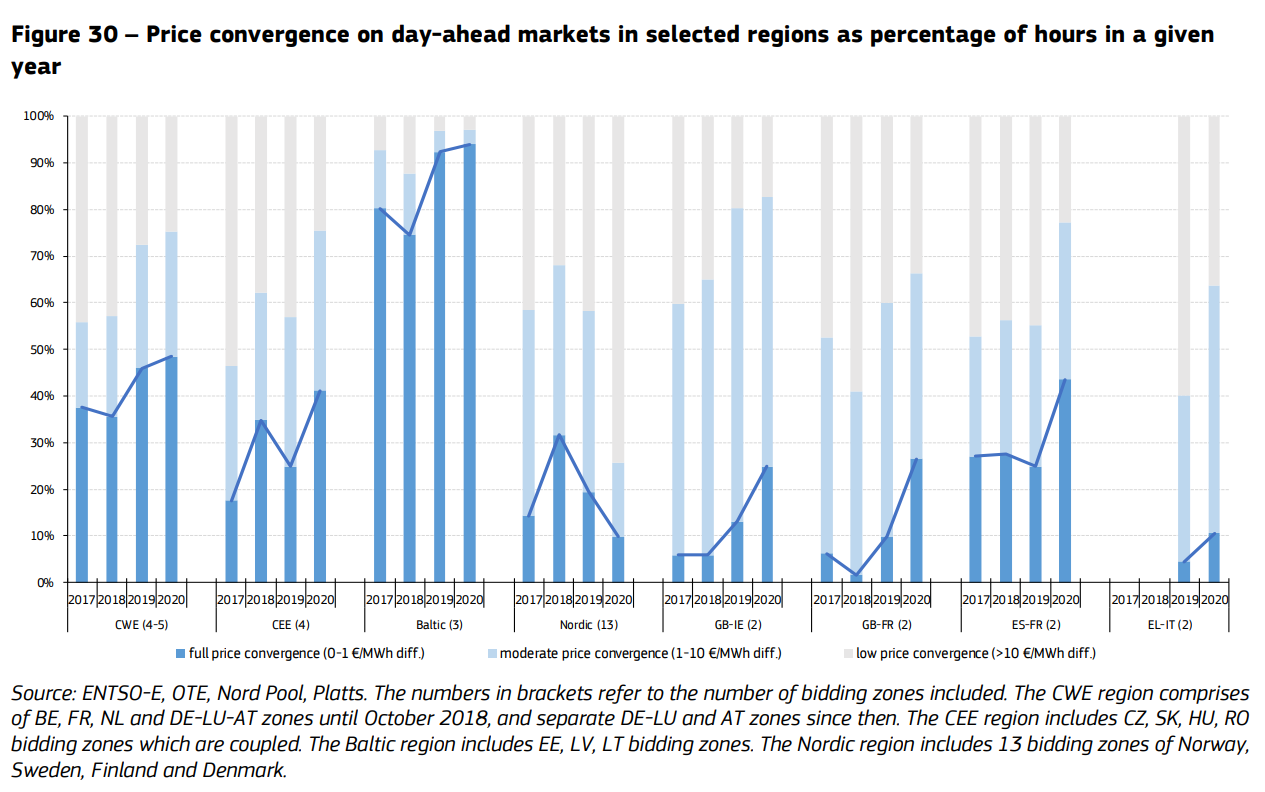
\includegraphics[height = 0.7\textheight]{figures/convergence.PNG}
        \caption{\cite{Report2019}}
    \end{figure}
\end{frame}

\begin{frame}[allowframebreaks]{Bibliography}
    \printbibliography
\end{frame}

\end{document}